\documentclass[tikz,border=12pt]{standalone}
\usepackage[utf8]{inputenc}
\usepackage{amssymb}
\usepackage{tikz}
\usetikzlibrary{shapes,arrows.meta,positioning,calc}

\definecolor{ScoutGreen}{HTML}{005432}
\definecolor{ScoutNavy}{HTML}{002855}
\definecolor{ScoutBlue}{HTML}{006EB6}
\definecolor{ScoutRed}{HTML}{A31920}
\definecolor{ScoutAmber}{HTML}{D97706}
\definecolor{BorderGray}{HTML}{CBD5E1}

\begin{document}
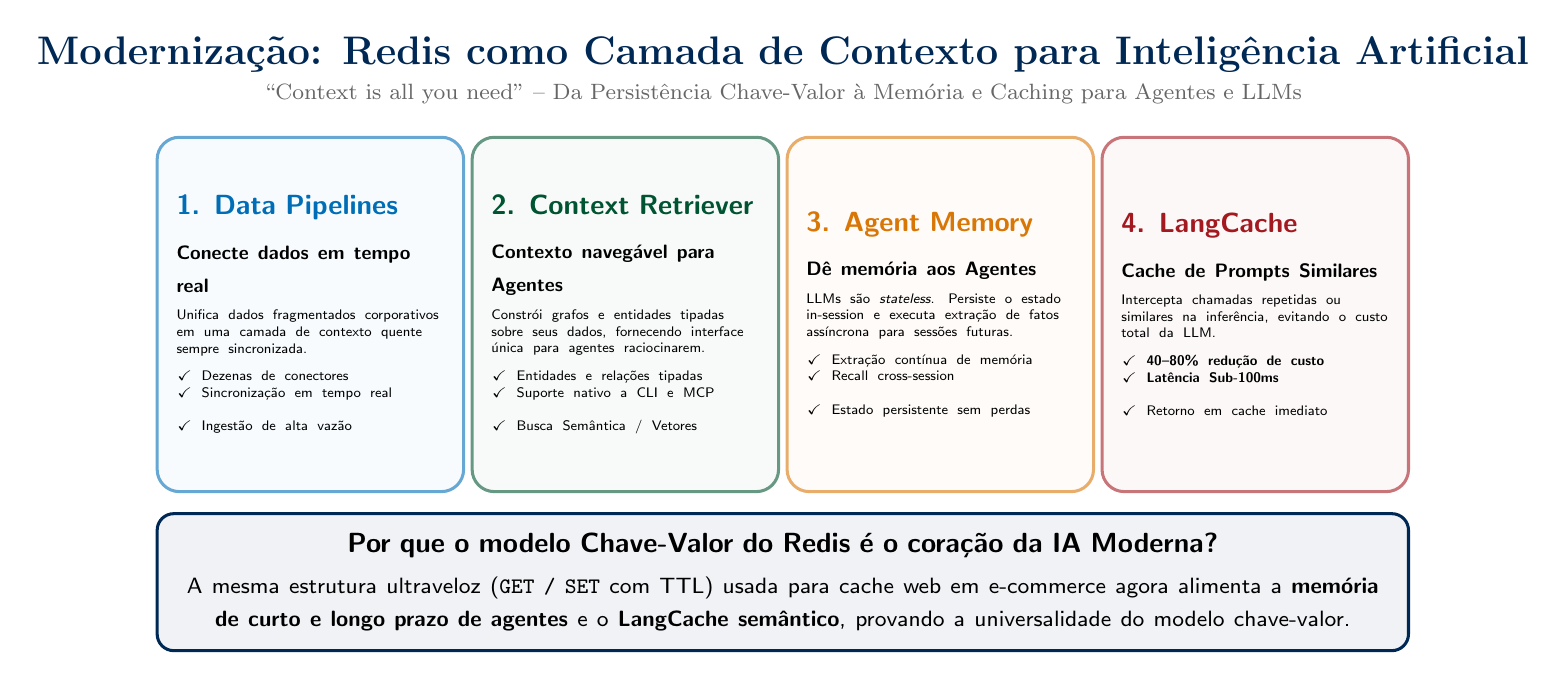
\begin{tikzpicture}[
    font=\sffamily,
    card/.style={draw=BorderGray, rounded corners=8pt, fill=white, line width=1.1pt, align=left, inner sep=7pt, minimum height=4.5cm, text width=3.4cm}
]

  % Cabeçalho
  \node[font=\bfseries\Large, text=ScoutNavy] at (7.8, 6.0) {Modernização: Redis como Camada de Contexto para Inteligência Artificial};
  \node[font=\footnotesize, text=gray!80!black] at (7.8, 5.5) {``Context is all you need'' -- Da Persistência Chave-Valor à Memória e Caching para Agentes e LLMs};

  % Card 1: Data Pipelines
  \node[card, draw=ScoutBlue!60, fill=ScoutBlue!3] (c1) at (1.8, 2.7) {
    \textbf{\textcolor{ScoutBlue}{1. Data Pipelines}}\\[4pt]
    \textbf{\scriptsize Conecte dados em tempo real}\\[4pt]
    \tiny Unifica dados fragmentados corporativos em uma camada de contexto quente sempre sincronizada.\\[4pt]
    \tiny $\checkmark$ Dezenas de conectores\\
    \tiny $\checkmark$ Sincronização em tempo real\\
    \tiny $\checkmark$ Ingestão de alta vazão
  };

  % Card 2: Context Retriever
  \node[card, draw=ScoutGreen!60, fill=ScoutGreen!3] (c2) at (5.8, 2.7) {
    \textbf{\textcolor{ScoutGreen}{2. Context Retriever}}\\[4pt]
    \textbf{\scriptsize Contexto navegável para Agentes}\\[4pt]
    \tiny Constrói grafos e entidades tipadas sobre seus dados, fornecendo interface única para agentes raciocinarem.\\[4pt]
    \tiny $\checkmark$ Entidades e relações tipadas\\
    \tiny $\checkmark$ Suporte nativo a CLI e MCP\\
    \tiny $\checkmark$ Busca Semântica / Vetores
  };

  % Card 3: Agent Memory
  \node[card, draw=ScoutAmber!60, fill=ScoutAmber!3] (c3) at (9.8, 2.7) {
    \textbf{\textcolor{ScoutAmber}{3. Agent Memory}}\\[4pt]
    \textbf{\scriptsize Dê memória aos Agentes}\\[4pt]
    \tiny LLMs são \textit{stateless}. Persiste o estado in-session e executa extração de fatos assíncrona para sessões futuras.\\[4pt]
    \tiny $\checkmark$ Extração contínua de memória\\
    \tiny $\checkmark$ Recall cross-session\\
    \tiny $\checkmark$ Estado persistente sem perdas
  };

  % Card 4: LangCache
  \node[card, draw=ScoutRed!60, fill=ScoutRed!3] (c4) at (13.8, 2.7) {
    \textbf{\textcolor{ScoutRed}{4. LangCache}}\\[4pt]
    \textbf{\scriptsize Cache de Prompts Similares}\\[4pt]
    \tiny Intercepta chamadas repetidas ou similares na inferência, evitando o custo total da LLM.\\[4pt]
    \tiny $\checkmark$ \textbf{40--80\% redução de custo}\\
    \tiny $\checkmark$ \textbf{Latência Sub-100ms}\\
    \tiny $\checkmark$ Retorno em cache imediato
  };

  % Faixa inferior de impacto
  \node[draw=ScoutNavy, fill=ScoutNavy!6, rounded corners=6pt, text width=15.4cm, align=center, line width=1.1pt, inner sep=7pt] at (7.8, -0.7) {
    \textbf{Por que o modelo Chave-Valor do Redis é o coração da IA Moderna?}\\[3pt]
    \footnotesize A mesma estrutura ultraveloz (\texttt{GET / SET} com TTL) usada para cache web em e-commerce agora alimenta a \textbf{memória de curto e longo prazo de agentes} e o \textbf{LangCache semântico}, provando a universalidade do modelo chave-valor.
  };

\end{tikzpicture}
\end{document}
